\documentclass[a4paper,UTF8]{article}
\usepackage{ctex}
\usepackage[margin=1.25in]{geometry}
\usepackage{color}
\usepackage{graphicx}
\usepackage{amssymb}
\usepackage{amsmath}
\usepackage{amsthm}
\usepackage{soul, color, xcolor}
\usepackage{bm}
\usepackage{tcolorbox}
\usepackage{hyperref}
\numberwithin{equation}{section}
%\usepackage[thmmarks, amsmath, thref]{ntheorem}
\theoremstyle{definition}
\newtheorem*{solution}{Solution}
\newtheorem*{prove}{Proof}
\usepackage{multirow}
\usepackage{diagbox}
\usepackage{float}

\setlength{\parindent}{0pt}
\newcommand{\bds}{\boldsymbol}
\def \X {\mathbf{X}}
\def \A {\mathbf{A}}
\def \C {\mathbf{C}}
\def \w {\hat{\boldsymbol{w}}}
\def \y {\mathbf{y}}
\def \x {\mathbf{x}}
\def \z {\mathbf{z}}
\def \hy {\widehat{y}}
\def \by {\Bar{y}}
\def \H {\mathbf{H}}
\def \I {\mathbf{I}}
\newcommand\given[1][]{\:#1\vert\:}


\begin{document}
\title{机器学习导论\ 习题二}
\author{学号, 姓名, \href{mailto:邮箱}{邮箱}}
\maketitle
\section*{作业提交注意事项}
\begin{tcolorbox}
	\begin{enumerate}
		\item[1.] 请在LaTeX模板中第一页填写个人的学号、姓名、邮箱;
		\item[2.] 本次作业需提交作答后的该 pdf 文件、编程题~.ipynb 文件; {\color{red}\textbf{请将二者打包为~.zip 文件上传}}. 注意命名规则, 三个文件均命名为 “$\text{学号}\_\text{姓名}$” + “.后缀” (例如 $\text{211300001}\_\text{张三}$” + “.pdf”、“.ipynb”、“.zip”);
		\item[3.] 若多次提交作业, 则在命名~.zip 文件时加上版本号, 例如 211300001\_张三\_v1.zip” (批改时以版本号最高的文件为准);
		\item[4.] 本次作业提交截止时间为 {\color{red}\textbf{ 4 月 19 日23:59:59}}. 未按照要求提交作业, 提交作业格式不正确, {\color{red}\textbf{作业命名不规范}}, 将会被扣除部分作业分数; 除特殊原因 (如因病缓交, 需出示医院假条) 逾期未交作业, 本次作业记 0 分; {\color{red}\textbf{如发现抄袭, 抄袭和被抄袭双方成绩全部取消}};
		\item[5.] 本次作业提交地址为 \href{https://box.nju.edu.cn/u/d/72f6f8cfff054611b6d3/}{here}, 请大家预留时间提前上交, 以防在临近截止日期时, 因网络等原因无法按时提交作业.
	\end{enumerate}
\end{tcolorbox}
\newpage


\section{[20pts] Linear Discriminant Analysis}
线性判别分析 (Linear Discriminant Analysis, 简称 LDA) 是一种经典的线性学习方法. 请仔细阅读《机器学习》第三章 3.4 节, 并回答如下问题.

\begin{enumerate}
	\item[(1)] \textbf{[10pts]} (二分类) 假设有两类数据, 其中正类服从高斯分布$P=\mathcal{N}\left(\bds{\mu}_1, \bds{\Sigma}_1\right)$, 负类服从高斯分布 $Q=\mathcal{N}\left(\bds{\mu}_2, \bds{\Sigma}_2\right)$. 对于任一样本 $\bds{x}$, 若分类器 $h$ 满足:
     $$
     h(\bds{x})= \begin{cases}0 & P(\bds{x})\leq Q(\bds{x}), \\ 1 & P(\bds{x})>Q(\bds{x}), \end{cases}
     $$
     则认为 $h$ 实现了最优分类. 假设 $\bds{\mu}_1,\bds{\mu}_2, \bds{\Sigma}_1, \bds{\Sigma}_2$ 均已知, 请证明当 $\bds{\Sigma}_1=\bds{\Sigma}_2=\bds{\Sigma}$ 时, 通过 LDA 得到的分类器可实现最优分类.
     (提示: 找到满足最优分类性质的分类平面)
	\item[(2)] \textbf{[10pts]} (多分类) 将 LDA 推广至多分类任务时, 可采用教材中式 (3.44) 作为优化目标. 通过求解式 (3.44), 可得到投影矩阵 $\mathbf{W}\in \mathbb{R}^{d\times d'}$, 其中 $d$ 为数据原有的属性数. 假设当前任务共有 $N$ 个类别, 请证明 $d'\leq N-1$. (提示: 对于任意 $n$ 阶方阵, 其非零特征值个数小于等于其秩大小)
\end{enumerate}


\begin{solution}
(1)书上公式3.39,得$w=\frac{1}{2} \Sigma^{-1} (\mu_1-\mu_2)$\\
两个类别在投影面连线的中点为$\frac{1}{2}(\mu_1+\mu_2)^T w=\frac{1}{4}(\mu_1+\mu_2)^T \Sigma^{-1} (\mu_1-\mu_2)$\\
对于$P(x)\leq Q(x)$,有$\frac{f_P(x)}{f_Q(x)}\leq 1 \quad$ f表示概率密度函数\\
\begin{align*}
&\ln \frac{f_1(\boldsymbol{x})}{f_2(\boldsymbol{x})}\\
&=-\frac{1}{2}(\boldsymbol{x}-\boldsymbol{\mu}_1)^T\boldsymbol{\Sigma}^{-1}(\boldsymbol{x}-\boldsymbol{\mu}_1)+\frac{1}{2}(\boldsymbol{x}-\boldsymbol{\mu}_2)^T\boldsymbol{\Sigma}^{-1}(\boldsymbol{x}-\boldsymbol{\mu}_2)\\
&= \boldsymbol{x}^T\boldsymbol{\Sigma}^{-1}(\boldsymbol{\mu}_2 - \boldsymbol{\mu}_1) + \frac{1}{2}\boldsymbol{\mu}_1^T\boldsymbol{\Sigma}^{-1}\boldsymbol{\mu}_1 - \frac{1}{2}\boldsymbol{\mu}_2^T\boldsymbol{\Sigma}^{-1}\boldsymbol{\mu}_2\\
&=\boldsymbol{x}^T\boldsymbol{\Sigma}^{-1}(\boldsymbol{\mu}_2 - \boldsymbol{\mu}_1)-\frac{1}{2}(\boldsymbol{\mu}_2+\boldsymbol{\mu}_1)^T\boldsymbol{\Sigma}^{-1}(\boldsymbol{\mu}_2-\boldsymbol{\mu}_1)\leq 0\\
\end{align*}
x在w上的投影更为接近靠近$\mu_2$在w上的投影,会被分类为0,对于$P(x)\geq Q(x)$同理,所以LDA找到的分类器是最优的\\
(2)考虑闭式解$S_w^{-1}S_b$的N-1个最大广义特征值对应的特征向量组成的矩阵\\
由于$\mbox{所有示类的均值向量}\mu=\frac{1}{N} \sum_{i=1}^{N}m_i \mu_i$所以可以把$\mu$融入群众中\\
$\frac{1}{N} \sum_{i=1}^{N}m_i (\mu_i-\mu)=0$\\在$S_b$中最多N-1个线性无关向量,比如说$\mu_2-\mu,\mu_3-\mu...,\mu_N-\mu$\\
由于$rank(S_w^{-1}S_b)\leq \min\{rank(S_w^{-1}),rank(S_b)\}\leq N-1$
秩至多为N-1,最多N-1个非0特征值对应的特征向量,W定义为$d \times d',d'\leq N-1$
\end{solution}

\newpage

\section{[20pts] Multi-Class Learning}
现实场景中我们经常会遇到多分类任务,处理思路主要分为两种:一是利用一些基本策略
(OvO,OvR,MvM),将多分类任务拆分为若干个二分类任务;二是直接求解,将常见的二分类学习器推广为多分类学习器. 请仔细阅读《机器学习》第三章3.5节,并回答如下问题.
\begin{enumerate}
	\item[(1)] \textbf{[5pts]}  考虑如下多分类学习问题:样本数量为$n$, 类别数量为$K$, 每个类别的样本数量一致. 假设一个二分类算法对于大小为$m$的数据训练的时间复杂度为$\mathcal{O}(m^\alpha)$, 试分别计算该算法在OvO、OvR策略下训练的总体时间复杂度.
	\item[(2)] \textbf{[5pts]}  当我们使用MvM处理多分类问题时,正、反类的构造需要有特殊的设计,一种最常用的技术是“纠错输出码"(ECOC). 考虑ECOC中的编码矩阵为“三元码”的形式,即在正、反类之外加入了“停用类”. 请通过构造具体的编码矩阵, 说明OvO、OvR均为此ECOC的特例.
	\item[(3)] \textbf{[10pts]}  对数几率回归(logistic regression)是一种常用的二分类模型, 简称对率回归. 现如今问题由二分类推广至多分类, 其中共有$K$个类别即$y \in \{1,2,\cdots, K\}$. 基于使用线性模型拟合对数几率这一思路, 请将对数几率回归算法拓展至多分类任务,
	给出该多分类对率回归模型的“对数似然”, 并给出该“对数似然”的梯度.

	提示1: 考虑如下$K-1$个对数几率, 分别用$K-1$组线性模型进行预测,
	\begin{align*}
		\ln{\frac{p(y=1 \given \x)}{p(y=K \given \x)}}, \ln{\frac{p(y=2 \given \x)}{p(y=K \given \x)}}, \cdots, \ln{\frac{p(y=K-1 \given \x)}{p(y=K \given \x)}}
	\end{align*}

	提示2: 定义指示函数$\mathbb{I}(\cdot)$使得答案简洁,
	\begin{align*}
		\mathbb{I}(y = j) = \begin{cases}
			0 & \text{若$y$不等于$j$} \\
			1 & \text{若$y$等于$j$}
		\end{cases}
	\end{align*}


\end{enumerate}


\begin{solution}
	此处用于写解答(中英文均可)
	~\\
	(1)OvO:$\frac{K(K-1)}{2}O((\frac{2n}{K})^{\alpha})$\\
	OvR:$KO(n^{\alpha})$\\
	(2)+1表示作为正例,-1表示作为反例,0表示不考虑\\
	OvO:每个分类器只考虑两个类,一个正例设置为+1,一个反例设置为-1,其余为0\\
	OvR:每个分类器只把一个类作为正例,设置为+1,其余类均设置为-1\\
	(3)\begin{align*}
		&z_j(x)=\w_j^T x+b_j,j=1,2,...K-1\\
		&z_K(x)=-\sum_{j=1}^{K-1} \w_j^T x-b_K\\
		&P(y=j|x)=\frac{exp(z_j(x))}{\sum_{k=1}^{K}exp(z_k(x))}\\
		&\mbox{对任意个样本xi,yi,目标是最大化对数似然函数}\\
		&L(w)=\sum_{i=1}^{N} \ln(P(y=y_i|x_i))\\
		&\mbox{对于j=1,2,...K-1}\\
		&\frac{\partial L(w)}{\partial w_j}=\sum_{i=1}^{N} [x_i (I(y_i=j)-P(y=j|x_i))]\\
		&\mbox{对于j=K}\\
		&\frac{\partial L(w)}{\partial w_K}=\sum_{i=1}^{N} [x_i (I(y_i=K)-P(y=K|x_i))]-\sum_{j=1}^{K-1}\frac{exp(z_j(x))}{\sum_{k=1}^{K-1}exp(z_k(x))+1}x_i\\
	\end{align*}
	~\\
\end{solution}

\newpage

\section{[20pts] Decision Tree Analysis}
决策树在实际应用中的性能虽然不及深度神经网络等复杂模型,但其可以作为弱学习器,在强大的集成算法如XGBoost中发挥重要的作用. 假设分类问题中标记空间 $\mathcal{Y}$ 的大小为$|\mathcal{Y}|$,训练集D中第$k$类样本所占比例为$p
_k(k=1,2,\cdots,|\mathcal{Y}|)$,请仔细阅读《机器学习》第四章, 并回答如下问题.
\begin{enumerate}
	\item[(1)] \textbf{[5pts]} 给定离散随机变量$X$和$Y$,条件熵(conditional entropy)$H(Y|X)$定义如下:
	\begin{align*}
		H(Y|X) = -\sum_{x}P(x)H(Y|X=x) = -\sum_{x}P(x)\sum_{y}P(y|x)\log_2 P(y|x),
	\end{align*}
	诠释为$Y$中不依赖$X$的信息量;$X$和$Y$的互信息(mutual information)定义如下:
	\begin{align*}
		I(X;Y) = \sum_{x,y} P(x,y) \log_2 \frac{P(x,y)}{P(x)P(y)}.
	\end{align*}
	请证明$I(X;Y) = H(X) - H(X|Y) = H(Y) - H(Y|X) \geq 0$,给出等号成立的条件,并用一句话描述互信息的含义.
	(提示: 使用Jensen不等式)
	\item[(2)] \textbf{[5pts]} 在ID3决策树的生成过程中,使用信息增益(information gain)为划分指标以生成新的结点.试证明或给出反例:在ID3决策树中, 根结点处划分的信息增益不小于其他结点处划分的信息增益.
	\item[(3)] \textbf{[5pts]} 设离散属性$a$有$V$种可能的取值$\{a^1,\cdots,a^V\}$, 请使用《机器学习》4.2.1节相关符号证明:
	\begin{align*}
		\text{Gain}(D,a) = \text{Ent}(D) - \sum_{v=1}^V \frac{\lvert D^v\rvert}{\lvert D \rvert} \text{Ent}(D^v) \geq 0
	\end{align*}
	即信息增益是非负的. (提示: 将信息增益表示为互信息的形式,你需要定义表示分类标记的随机变量,以及表示属性$a$取值的随机变量)
	\item[(4)] \textbf{[5pts]} 除教材中介绍的信息熵、基尼指数(gini index)外, 也可以使用误分类错误率(misclassification error)
	\begin{align*}
		1 - \max_{k} p_k
	\end{align*}
	作为衡量集合纯度的指标. 请从决策树生成过程的角度给出这一指标的合理性,并结合二分类问题($\lvert \mathcal{Y} \rvert = 2$)下三种纯度指标的表达式,分析各衡量标准的特点.
\end{enumerate}

\begin{solution}
此处用于写解答(中英文均可)
~\\
(1)琴生不等式$f(E[X]) \leq E[f(x)]$其中f是凸函数,所以不妨带入f(x)=-log(x)\\
得到$-log(E[X]) \leq E[-log(X)]$\\
\begin{align*}
	I(X;Y) &= \sum_{x,y} P(x,y) \log_2 \frac{P(x,y)}{P(x)P(y)}\\
	&= \sum_{x,y} P(x,y)(\log_2 P(x,y)-\log_2 P(x)-\log_2 P(y))\\
	&=\sum_{x,y} P(x,y)\frac{\log_2 P(x,y)}{\log_2 P(x)}-\sum_{x,y} P(x,y)\log_2 P(y)\\
	&=H(Y)-H(Y|X)\\
	&=\sum_{x,y} P(x,y)\frac{\log_2 P(x,y)}{\log_2 P(y)}-\sum_{x,y} P(x,y)\log_2 P(x)\\
	&=H(X)-H(X|Y)\\
	I(X;Y) &= \sum_{x,y} P(x,y) \log_2 \frac{P(x,y)}{P(x)P(y)}\\
	&=E[\frac{P_{x,y}(x,y)}{P_x(x)P_y(y)}]\\
	&=E[-\log \frac{P_x(x)P_y(y)}{P_{x,y}(x,y)}]\\
	&\geq -log (E[\frac{P_x(x)P_y(y)}{P_{x,y}(x,y)}])=-\log 1=0
\end{align*}
(2)不正确\\
就考虑课本上76,77页西瓜数据集2.0的例子,根节点纹理划分后,信息增益0.381,而使用根蒂对清晰分支划分后信息增益为0.458,这是一个反例\\
(3)记表示分类的随机变量为Y,表示属性a取值的随机变量为A\\
\begin{align*}
	\text{Gain}(D,a) &= \text{Ent}(D) - \sum_{v=1}^V \frac{\lvert D^v\rvert}{\lvert D \rvert} \text{Ent}(D^v)\\
	&=-\sum_{y}P(Y=y)\log_2 P(Y=y)+\sum_{a}P(A=a)\sum_{y}P(y|a)\log_2 P(y|a)\\
	&=H(Y)-H(Y|A)=I(Y;A) \geq 0
\end{align*}
~\\
\end{solution}

\newpage

\section{[20pts] Training a Decision Tree}
剪枝(pruning)是决策树学习算法对抗“过拟合”的主要手段.考虑下面的训练集:共计8个训练样本,每个训练样本有三个特征属性$X,Y,Z$和标签信息.详细信息如表\ref{problem2_training_set}所示.
\begin{table}[ht]
    \centering
	\setlength{\abovecaptionskip}{0pt}
	\setlength{\belowcaptionskip}{5pt}
    \caption{训练集信息}
	\label{problem2_training_set}
    %\tabcolsep 15pt
    \begin{tabular}{cccc|c||cccc|c}
        \hline 
        编号 & $X$ & $Y$ & $Z$ & $f$ & 编号 & $X$ & $Y$ & $Z$ & $f$ \\
    \hline1 &   1 &  1 &   0 &   1 &   5 &    0 &   0 &   0 &   0\\
          2 &   1 &  1 &   1 &   1 &   6 &    1 &   0 &   1 &   0 \\
          3 &   0 &  0 &   1 &   0 &   7 &    1 &   1 &   0 &   1\\
          4 &   0 &  1 &   0 &   0 &   8 &    0 &   1 &   1 &   1\\
        \hline
    \end{tabular}
\end{table}
\begin{enumerate}
	\item[(1)] \textbf{[5pts]} 请通过训练集中的数据训练决策树,要求使用“信息增益”(information gain)作为划分准则.(需说明详细计算过程)
	\item[(2)] \textbf{[10pts]} 进一步考虑如表\ref{problem2_validation_set}所示的验证集,对上一问得到的决策树基于这一验证集进行预剪枝、后剪枝.生成叶子结点时,若样例最多的类别不唯一,可任选其中一类.请画出所有可能的剪枝结果.(需说明详细计算过程)
	\begin{table}[ht]
		\centering
		\setlength{\abovecaptionskip}{0pt}
		\setlength{\belowcaptionskip}{5pt}
		\caption{验证集信息}
		\label{problem2_validation_set}
		\begin{tabular}{cccc|c}
		\hline
		编号 & $X$ & $Y$ & $Z$ & $f$ \\ \hline
		  9 &   1 &   1&   1&    1\\
		  10 &   1&    0&   1&    0\\
		  11 &   1&    0&   1&    1\\
		  12 &   0&    1&   0&    0\\
		  13 &   0&    1&   1&    1\\
		  14 &   1&    0&   0&    0\\ \hline
		\end{tabular}
	\end{table}
	\item[(3)] \textbf{[5pts]}请给出预剪枝决策树和后剪枝决策树分别在训练集、验证集上的准确率. 结合本题的结果,讨论预剪枝与后剪枝在欠拟合风险、泛化能力以及训练时间开销层面各自的特点. 
\end{enumerate}


\newpage
\begin{solution}
此处用于写解答(中英文均可)
~\\
(1)
\begin{align*}
	&Ent(D)=-(0.5\log_2(0.5)+0.5 \log_2(0.5))=1\\
	&Gain(D,X)=1+(0.5(0.75 \log_2 0.75+0.25 \log_2 0.25)+0.5(0.75 \log_2 0.75+0.25 \log_2 0.25))=0.1887\\
	&Gain(D,Y)=1+(\frac{3}{8}\times0+\frac{5}{8}(0.2\log_2 0.5+0.8 \log_2 0.8))=0.5488\\
	&Gain(D,Z)=1+(\frac{1}{2}(\frac{1}{2}\log_2 \frac{1}{2}+\frac{1}{2}\log_2 \frac{1}{2})+\frac{1}{2}(\frac{1}{2}\log_2 \frac{1}{2})+\frac{1}{2}\log_2 \frac{1}{2})=0\\
	&\mbox{选Y进行划分,Y=0对应的3,5,6样例均是负例,Y=1对应的1,2,4,7,8中4
	是负例,其余是正例,再划分}\\
	&Ent(D')=0.8\log_20.8+0.2\log_20.2=0.7219\\
	&Gain(D',X)=0.7219+(0+0.4(\frac{1}{2}\log_2 \frac{1}{2})+\frac{1}{2}\log_2 \frac{1}{2}))=0.3219\\
	&Gain(D',Z)=0.7219+(0+0.6(\frac{2}{3}\log_2 \frac{2}{3}+\frac{1}{3}\log_2\frac{1}{3}))=0.1709\\
	&\mbox{再选X进行划分X=0对应4,8一正例一负例,X=1对应1,2,7都是正例}\\
	&\mbox{最后选Z进行划分Z=0对应负例,Z=1对应正例}\\
\end{align*}
\begin{figure}[htbp]
	\centering
	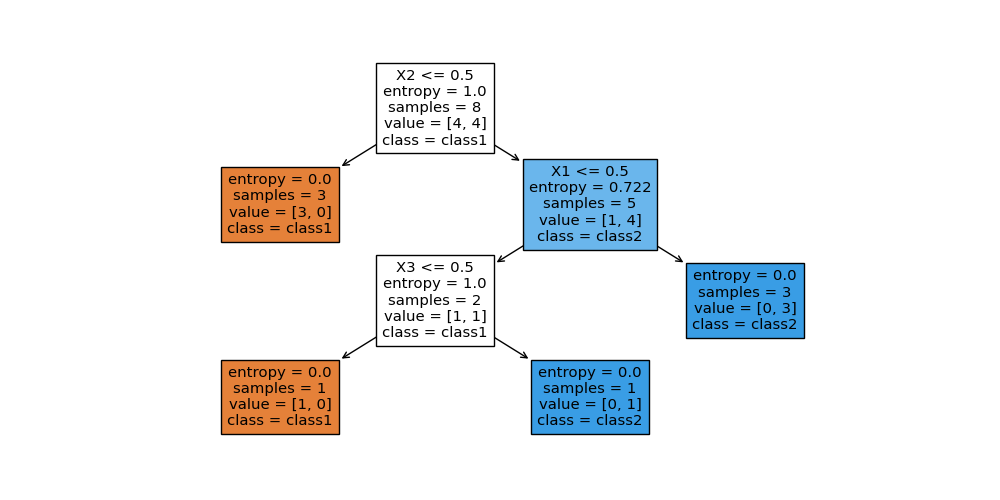
\includegraphics[scale=0.7]{Q4tree.png}
\end{figure}\\
(2)预剪枝:对Y划分前测试集准确率$50\% $,划分后准确率$\frac{2}{3}$(11,12预测错误)进行划分\\
对X划分前测试集准确率$\frac{2}{3}$(11,12预测错误),划分后准确率$\frac{2}{3}$(11,13预测错误),禁止划分\\
\begin{figure}[htbp]
	\centering
	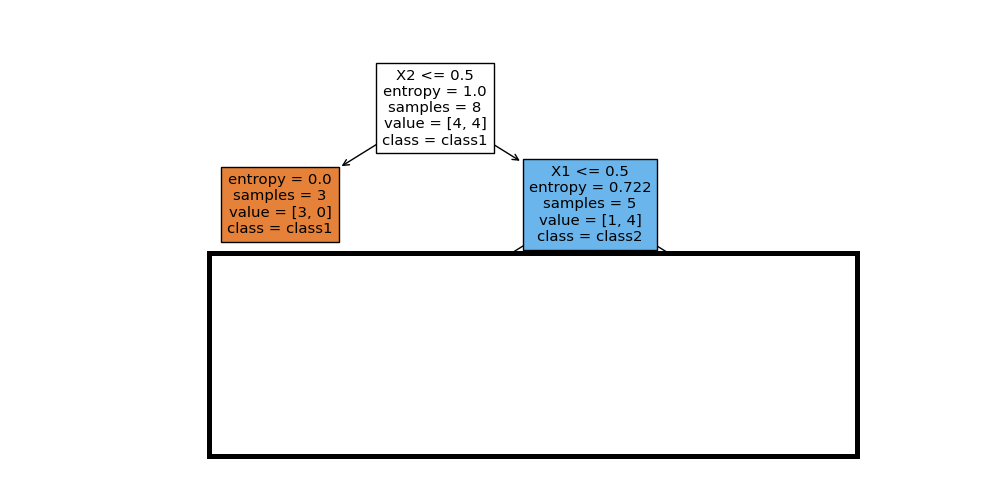
\includegraphics[scale=0.7]{Q4tree(2)1.png}
\end{figure}\\
后剪枝:看是否以Z进行划分,剪枝前准确率$\frac{5}{6}$(11预测错误),剪枝后准确率$\frac{2}{3}$(11,13预测错误),所以不剪枝最终结果和(1)中一样\\
\begin{figure}[htbp]
	\centering
	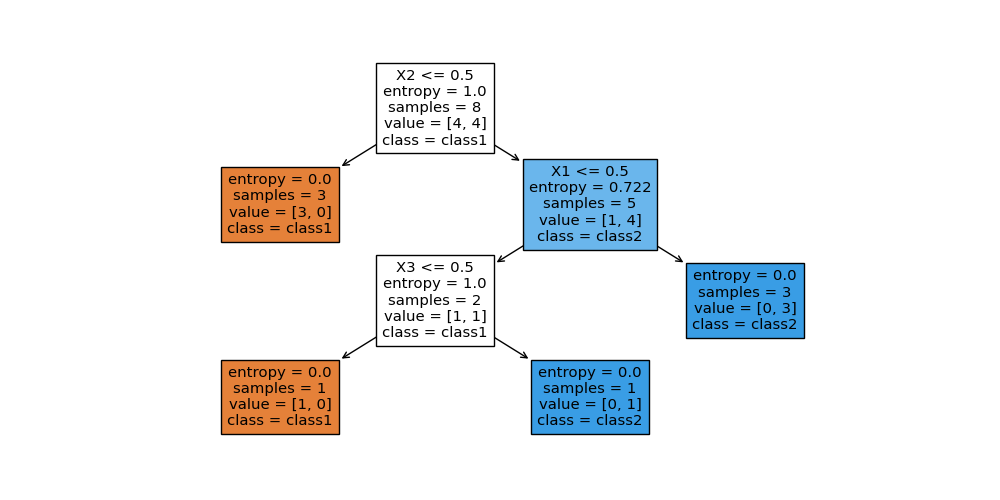
\includegraphics[scale=0.7]{Q4tree.png}
\end{figure}
~\\
\end{solution}

\newpage

\section{[20pts] Kernel Function}
核函数是 SVM 中常用的工具,其在机器学习中有着广泛的应用与研究. 请自行阅读学习《机器学习》第 6.3 节, 并回答如下问题.
\begin{enumerate}
	\item[(1)] \textbf{[5pts]} 试判断 $\kappa(\x, \z) = \left(\langle\x, \z\rangle - 1\right)^2$ 是否为核函数,并给出证明或反例.
	\item[(2)] \textbf{[5pts]} 试证明:对于半正定矩阵 $\A$,总存在半正定矩阵 $\C$,成立$\A = \C^\top \C$
	\item[(3)] \textbf{[5pts]} 试证明:若 $\kappa_1$ 和 $\kappa_2$ 为核函数, 则两者的直积
	\[
	\kappa_1 \otimes \kappa_2(\x, \z)=\kappa_1(\x, \z) \kappa_2(\x, \z)
	\]
	也是核函数;
	\item[(4)] \textbf{[5pts]} 试证明 $\kappa(\x, \z) = \langle\x, \z\rangle^p$ 对 $\forall p\in\mathbb{Z}_+(p<\infty)$ 均为核函数.

	
\end{enumerate}

\begin{solution}
此处用于写解答(中英文均可)
~\\
(1)不是,$\x_1=(-1,1),\x_2=(-1,-1)$\\
$$
K=\begin{pmatrix}
	-2&-1\\
	-1&0
\end{pmatrix}
$$
$$
\begin{pmatrix}
	1&1
\end{pmatrix}
\begin{pmatrix}
	-2&-1\\
	-1&0
\end{pmatrix}
\begin{pmatrix}
	1\\
	1
\end{pmatrix}=-4<0
$$
所以核矩阵不是半正定的,$\kappa$不是核函数\\
(2)半正定矩阵是对称的,考虑$\A=\C ^2$\\
对A特征值分解得到$A=Q\Sigma Q^{-1}$\\
其中$\Sigma$的对角线上为半正定矩阵A的特征值\\
记一个矩阵$\Sigma'$,其对角线上的元素为$\Sigma$对角线上元素的0.5次方\\
令$C=Q\Sigma' Q^{-1}$,则$C^2=Q\Sigma' Q^{-1}Q\Sigma' Q^{-1}=Q\Sigma Q^{-1}=A$\\
而且C显然也是半正定矩阵,所以$C=C^T$,所以$A=C^T C$\\
(3)
\begin{align*}
\kappa_1 \otimes \kappa_2(\x, \z)&=\kappa_1(\x, \z) \kappa_2(\x, \z)\\
&=(\Phi_1 (x)^T \Phi_1 (z))(\Phi_2 (x)^T \Phi_2 (z))\\
&=\sum_{t=1}^{m}(\Phi_{1t}(x)\Phi_{2t}(x)\Phi_{1t}(z)\Phi_{2t}(z))\\
&=\Phi(x)^T\Phi(z)\\
\end{align*}
(4)我觉得可以数学归纳法,因为$<\x,\z>$是线性核\\
当p=1时成立,假设当p=k时结论成立\\
当p=k+1时,$<x,z>^{k+1}=<x,z>^{k} <x,z>$视作了两个核函数的直积\\
根据(3)可知p=k+1时,也是核函数,所以 $\kappa(\x, \z) = \langle\x, \z\rangle^p$ 对 $\forall p\in\mathbb{Z}_+(p<\infty)$ 均为核函数.
\end{solution}



\end{document}